%%
%% Copyright 2007-2020 Elsevier Ltd
%%
%% This file is part of the 'Elsarticle Bundle'.
%% ---------------------------------------------
%%
%% It may be distributed under the conditions of the LaTeX Project Public
%% License, either version 1.2 of this license or (at your option) any
%% later version.  The latest version of this license is in
%%    http://www.latex-project.org/lppl.txt
%% and version 1.2 or later is part of all distributions of LaTeX
%% version 1999/12/01 or later.
%%
%% The list of all files belonging to the 'Elsarticle Bundle' is
%% given in the file `manifest.txt'.
%%
%% Template article for Elsevier's document class `elsarticle'
%% with harvard style bibliographic references

% For submission:
\documentclass[final,5p,times,twocolumn,authoryear]{elsarticle}

%% Use the option review to obtain double line spacing
% \documentclass[authoryear,preprint,review,12pt]{elsarticle}

%% Use the options 1p,twocolumn; 3p; 3p,twocolumn; 5p; or 5p,twocolumn
%% for a journal layout:
%% \documentclass[final,1p,times,authoryear]{elsarticle}
%% \documentclass[final,1p,times,twocolumn,authoryear]{elsarticle}
%% \documentclass[final,3p,times,authoryear]{elsarticle}
%% \documentclass[final,3p,times,twocolumn,authoryear]{elsarticle}
%% \documentclass[final,5p,times,authoryear]{elsarticle}
%% \documentclass[final,5p,times,twocolumn,authoryear]{elsarticle}

%% For including figures, graphicx.sty has been loaded in
%% elsarticle.cls. If you prefer to use the old commands
%% please give \usepackage{epsfig}

%% The amssymb package provides various useful mathematical symbols
\usepackage{amssymb}
\usepackage{amsmath}
%% The amsthm package provides extended theorem environments
%% \usepackage{amsthm}

%% The lineno packages adds line numbers. Start line numbering with
%% \begin{linenumbers}, end it with \end{linenumbers}. Or switch it on
%% for the whole article with \linenumbers.
%% \usepackage{lineno}

\graphicspath{{figures/}}
% imports
\usepackage{xcolor}
\usepackage{hyperref}
\hypersetup{
    colorlinks=true,
    linkcolor=black,
    filecolor=black,
    urlcolor=navy,
    citecolor=black,
}
\urlstyle{same}

% Packages / projects / programming
\newcommand{\package}[1]{\texttt{#1}}
\newcommand{\acronym}[1]{{#1}}
\newcommand{\github}{\textsl{GitHub}}
\newcommand{\python}{\textsl{Python}}
\newcommand{\jax}{\package{JAX}}
\newcommand{\agama}{\package{Agama}}
\newcommand{\gala}{\package{gala}}

% Missions
\newcommand{\gaia}{\textsl{Gaia}}
\newcommand{\hipparcos}{\textsl{HIPPARCOS}}
\newcommand{\dr}[1]{\acronym{DR}#1}
\newcommand{\apogee}{\acronym{APOGEE}}
\newcommand{\sdss}{\acronym{SDSS}}
\newcommand{\sdssiv}{\acronym{SDSS-IV}}

% Stats / probability
\newcommand{\given}{\,|\,}
\newcommand{\norm}{\mathcal{N}}
\newcommand{\pdf}{\textsl{pdf}}

% Maths
\newcommand{\dd}{\mathrm{d}}
\newcommand{\deriv}[2]{\frac{\mathrm{d}{#1}}{\mathrm{d}{#2}}}
\newcommand{\dderiv}[2]{\frac{\mathrm{d^2}{#1}}{\mathrm{d}{#2}^2}}
\newcommand{\Deriv}[2]{\frac{\mathrm{D}{#1}}{\mathrm{D}{#2}}}
\newcommand{\pderiv}[2]{\frac{\partial {#1}}{\partial {#2}}}
\newcommand{\ppderiv}[2]{\frac{\partial^2 {#1}}{\partial {#2}^2}}
\newcommand{\transpose}[1]{{#1}^{\mathsf{T}}}
\newcommand{\inverse}[1]{{#1}^{-1}}
\newcommand{\argmin}{\operatornamewithlimits{argmin}}
\newcommand{\mean}[1]{\left< #1 \right>}

% Non-scalar variables
\renewcommand{\vec}[1]{\ensuremath{\bs{#1}}}
\newcommand{\mat}[1]{\ensuremath{\mathbf{#1}}}

% Units:
% Workaround for siunitx + AASTeX
% https://tex.stackexchange.com/questions/192610/use-emulateapj-aastex-with-siunitx
\usepackage{savesym}
\savesymbol{tablenum}
\usepackage{siunitx}
\ifdefined\unit\else
  \ifdefined\NewCommandCopy
    \NewCommandCopy\unit\si
  \else
    \NewDocumentCommand\unit{O{}m}{\si[#1]{#2}}
  \fi
\fi
\restoresymbol{SIX}{tablenum}
\DeclareSIUnit\year{yr}
\DeclareSIUnit\parsec{pc}
\DeclareSIUnit\mag{mag}
\DeclareSIUnit\Msun{M_\odot}
\DeclareSIUnit\msun{M_\odot}
\DeclareSIUnit\Rsun{R_\odot}
\DeclareSIUnit\mas{mas}
\newcommand{\mas}{\unit{\milli\arcsecond}}
\newcommand{\muas}{\unit{\micro\arcsecond}}
\newcommand{\kms}{\unit{\km\per\s}}
\newcommand{\masyr}{\unit{\mas\per\year}}
\newcommand{\kpc}{\unit{\kilo\parsec}}
\newcommand{\usurfdens}{\unit{\msun.\parsec^{-2}}}
\newcommand{\uvoldens}{\unit{\msun.\parsec^{-3}}}

% Misc. formatting
\newcommand{\bs}[1]{\boldsymbol{#1}}

% Astronomy
\newcommand{\abun}[2]{\ensuremath{{[\mathrm{#1}/\mathrm{#2}]}}}
\newcommand{\feh}{\abun{Fe}{H}}
\newcommand{\afe}{\abun{\alpha}{Fe}}
\newcommand{\mgfe}{\abun{Mg}{Fe}}
\newcommand{\logg}{\ensuremath{\log g}}
\newcommand{\Teff}{\ensuremath{T_{\textrm{eff}}}}
\newcommand{\vsini}{\ensuremath{v\,\sin i}}

% Dynamics
\newcommand{\df}{\acronym{DF}}
\newcommand{\zmax}{\ensuremath{z_{\textrm{max}}}}

% TO DO
\newcommand{\todo}[1]{{\color{red} TODO: #1}}
\newcommand{\placeholder}[1]{{\color{purple} #1}}


\journal{New Astronomy Reviews}

\begin{document}

\begin{frontmatter}

%% Title, authors and addresses

%% use the tnoteref command within \title for footnotes;
%% use the tnotetext command for theassociated footnote;
%% use the fnref command within \author or \affiliation for footnotes;
%% use the fntext command for theassociated footnote;
%% use the corref command within \author for corresponding author footnotes;
%% use the cortext command for theassociated footnote;
%% use the ead command for the email address,
%% and the form \ead[url] for the home page:
%% \title{Title\tnoteref{label1}}
%% \tnotetext[label1]{}
%% \author{Name\corref{cor1}\fnref{label2}}
%% \ead{email address}
%% \ead[url]{home page}
%% \fntext[label2]{}
%% \cortext[cor1]{}
%% \affiliation{organization={},
%%            addressline={},
%%            city={},
%%            postcode={},
%%            state={},
%%            country={}}
%% \fntext[label3]{}

\title{Stellar Streams in the Gaia Era}

%% use optional labels to link authors explicitly to addresses:
%% \author[label1,label2]{}
%% \affiliation[label1]{organization={},
%%             addressline={},
%%             city={},
%%             postcode={},
%%             state={},
%%             country={}}
%%
%% \affiliation[label2]{organization={},
%%             addressline={},
%%             city={},
%%             postcode={},
%%             state={},
%%             country={}}

\author[ociw]{Ana~Bonaca}
\author[cca]{Adrian~M.~Price-Whelan}

\affiliation[ociw]{organization={The Observatories of the Carnegie Institution for Science},
            addressline={813 Santa Barbara Street},
            city={Pasadena},
            postcode={91101},
            state={CA},
            country={USA}}

\affiliation[cca]{
    organization={Center for Computational Astrophysics, Flatiron Institute},
    addressline={162 Fifth Ave.},
    city={New York},
    postcode={10010},
    state={NY},
    country={USA}
}


\begin{abstract}
- streams, tidal debris, useful for tracing hierarchical assembly, dark matter
- in the Milky Way, the Gaia mission, providing astrometry and spectrophotometry for billions of stars, fundamentally changed the landscape
- we discuss three main revolutions:
-- number of streams increased by an order of magnitude, now have a population of 100 (New streams and methods for discovery thanks to new kinds of data)
-- orbital histories (including hierarchical associations between streams)
-- Stream features are abundant (revealed at low surface brightness)
Implications heralding exciting times ahead!
-- pragmatic: Due to more secure membership probabilities, follow-up now more efficient so the chemistries now becoming more readily available
-- Due to large number of streams, transitioning from stamp-collecting to population studies
-- All of this will need improved theoretical modeling of the new Gaia discoveries
\end{abstract}

% %%Graphical abstract
% \begin{graphicalabstract}
% %\includegraphics{grabs}
% \end{graphicalabstract}
%
% %%Research highlights
% \begin{highlights}
% \item Research highlight 1
% \item Research highlight 2
% \end{highlights}

\begin{keyword}
%% keywords here, in the form: keyword \sep keyword

%% PACS codes here, in the form: \PACS code \sep code

%% MSC codes here, in the form: \MSC code \sep code
%% or \MSC[2008] code \sep code (2000 is the default)

\end{keyword}

\end{frontmatter}

%% \linenumbers

%% main text
\section{Introduction}
\label{sec:intro}
% AB
% storytelling prose

The \gaia\ mission has mapped the positions and motions of almost two billion stars in the Milky Way \citep{gaiamission:2016, gaiadr1, gaiadr2, gaiaedr3, gaiadr3}, so it comes as no surprise that it has fundamentally changed our view of stars that move on similar orbits---stellar streams.
Heralding from the lowest-mass stellar systems, and orbiting in the most dark-matter dominated regions of a galaxy, streams provide unique insights into physics of star and galaxy formation \citep{smith:2016, ferguson:2016, carlin:2016}, and the nature of dark matter \citep{johnston:2016a, johnston:2016b}.
So far, the main limitation for studying stellar streams in the Milky Way has been uncovering member stars of these low-mass and diffuse systems in the ocean of field stars.
\gaia\ proper motions have largely lifted this limitation, and as a result, maps of stellar streams in the \gaia\ era build a more complete picture of our Galaxy, its constituents and its history.

We center this review on three major breakthroughs that \gaia\ brought to stellar streams.
The first is the sheer number of stream discoveries, which \gaia\ increased by an order of magnitude from $\approx10$ to $\approx100$ (\S\ref{sec:discovery}).
The second is the detailed structure of stellar streams, resolved by \gaia\ for the first time to suggest dynamical histories rich in perturbations (\S\ref{sec:structure}).
And finally, the third are the stream kinematics, which constrained their precise orbits, as well as origins (\S\ref{sec:orbits}).
In these sections we also discuss the key opportunities and new research directions that these breakthroughs have made possible.
In the concluding section, we reflect more broadly on what these developments entail for the future of Galactic archaeology (\S\ref{sec:outlook}).
As for the remainder of this section, the last review dedicated to stellar streams was almost a decade ago and pre-\gaia\ \citep{newberg:2016}, while a more recent, \gaia-based review focused on the Milky Way's halo more broadly \citep{helmi:2020}, so we now proceed to outline the theoretical and historical context for \gaia's stellar stream revolution.

\begin{figure*}[t!]
\begin{center}
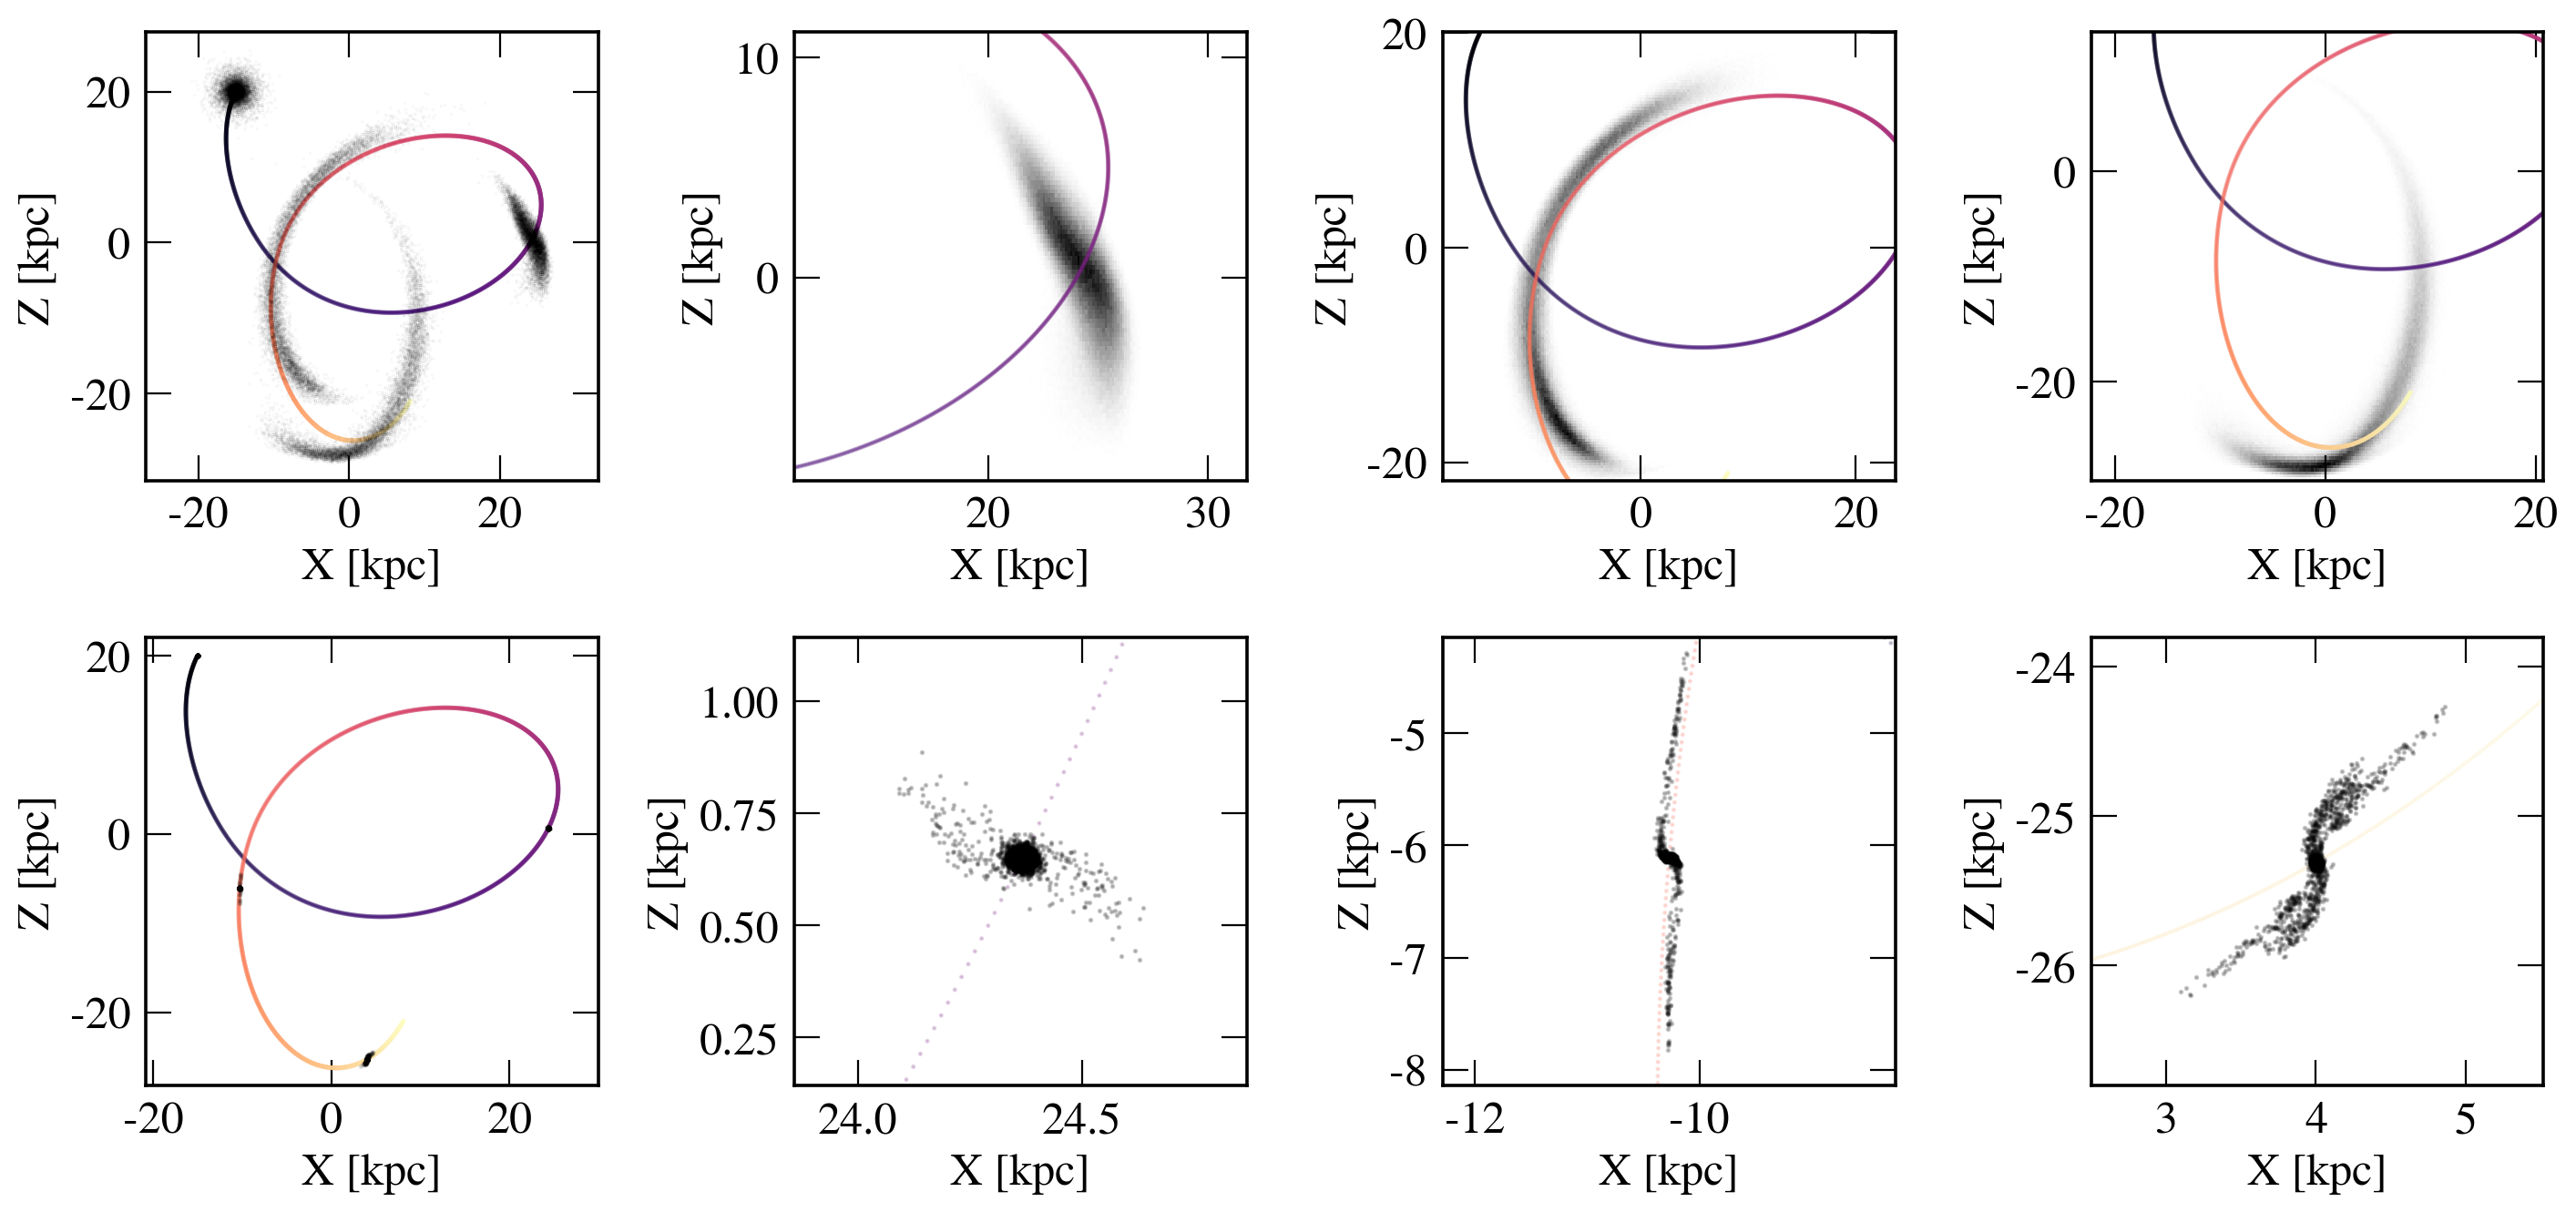
\includegraphics[width=1\textwidth]{figures/stream_formation.png}
\end{center}
\caption{%
A comparison of tidal tails with a dwarf galaxy (top) and a globular cluster progenitor (bottom).
\label{fig:stream_formation}
}
\end{figure*}

Physics driving the formation of stellar streams rests with the tidal forces of a host galaxy acting on its satellites.
When sufficiently strong, these tides pull stars out of the satellite through two stationary points \citep{bt:2008}, thus forming the leading tidal tail (stars with shorter orbital periods speeding ahead of the progenitor) and the trailing tidal tail (stars lagging behind the progenitor due to their longer orbital periods).
We illustrate the process of tidal dissolution in Figure~\ref{fig:stream_formation}, with a dwarf galaxy satellite at the top, and a globular cluster on a matching orbit at the bottom.
The dwarf galaxy of an initial mass of $10^8\,\unit{\msun}$ was represented with 50,000 particles and evolved with the Gyrfalcon tree code \citep{dehnen:2014}.
The globular cluster of an initial mass of $10^4\,\unit{\msun}$, was represented with 500,000 particles and modeled with direct N-body code PeTar \citep{wang:2020}.
The left-most panels show an early stage of dissolution, with short tails of gravitationally unbound stars emanating from each progenitor.
The boundary between the bound and unbound stars is set by the tidal radius.
Typically, the satellite mass $m$ is much smaller than the enclosed mass of the host galaxy at its location $M(<R_0)$, so the tidal radius is approximately the Jacobi radius from the restricted three-body problem \citep[][]{szebehely:1967, valtonen:2006}:
\begin{equation}
r_J = \left(\frac{m}{3M(<R_0)}\right)^{1/3} R_0
\end{equation}
The Jacobi radius, shown with a red dashed line in Figure~\ref{fig:stream_formation}, matches well the tidal boundary of both the globular cluster and the dwarf galaxy derived through self-consistent numerical simulations.
This agreement has been used to develop fast methods for generating models of stellar streams by placing tracer particles at the progenitor's Jacobi radius, and then solving the restricted three-body problem \citep[the so-called \emph{particle-spray methods};][]{varghese:2011, lane:2012, kupper:2012, bonaca:2014, gibbons:2014, fardal:2015}.
% TODO: and methods for constraining the underlying gravitational field? Johnston 1996, Binney 2008, Eyre, APW+2013, 2014, etc.

Governed by the same underlying gravitational potential, tidal tails of a globular cluster and a dwarf galaxy on the same orbit have similar shape and orientation.
Notably, both streams delineate the progenitor's orbit at pericenter, but are misaligned at apocenter (left and middle panels in Figure~\ref{fig:stream_formation}), which means that representing a stream as an orbit is not always appropriate, no matter how tempting the computational speed-ups are \citep{eyre:2009, eyre:2011, sanders:2013a, sanders:2013b}.
On the other hand, it is obvious from Figure~\ref{fig:stream_formation} that a globular cluster and a dwarf galaxy produce markedly different streams: dwarf galaxy streams are longer, wider, and smoother than globular cluster streams.
The cause of this discrepancy is not just the difference in their initial masses, but also in their number density of stars.
In more diffuse dwarf galaxies, a higher fraction of stars find themselves outside of the tidal radius when it shrinks during a pericentric passage (Figure~\ref{fig:stream_formation}, top center).
Combined with a higher velocity dispersion due to a higher initial mass \citep[cf.][]{simon:2007, baumgardt:2019}, the resulting tails are more massive, wider and grow faster.
In contrast, more compact globular clusters maintain a tidal radius larger than its half-mass radius even at pericenter.
As a result, their mass loss is dominated by stars escaping through close two-body encounters, i.e., the process of two-body relaxation or evaporation \citep{gnedin:1997,vesperini:1997,baumgardt:2003}.
Mass loss being driven by an internal process means that stars escape a globular cluster with a small relative velocity and at an approximately constant rate.
Stars released uniformly along the orbital phase appear to be on epicycles around the progenitor's orbit.
Seen in projection, these epicycles form a regular pattern of over- and under-densities along the globular cluster tails \citep[Figure~\ref{fig:stream_formation}, bottom right;][]{kupper:2008, kupper:2010, just:2009}.
This pattern is absent from dwarf galaxy tails due to its episodic mass loss of kinematically hotter stars, which results in a fairly uniform density (Figure~\ref{fig:stream_formation} top right).

Early theoretical models of interacting galaxies showed that reproducing the various configurations of tail and bridge features seen in catalogs of interacting galaxies \citep{vorontsov-velyaminov:1959, arp:1966} is possible through gravity alone \citep{pfleiderer:1963, toomre:1972}.
Their tidal origin makes streams extremely powerful tracers of the underlying gravitation field and dark matter, which dominates the mass budget in most galaxies \citep[e.g.,][]{moster:2010, behroozi:2019}.
Theoretical studies showed that the phase space of stellar streams can be used to measure the mass and shape of a dark matter halo on large scales \citep{springel:1999, dubinski:1999}, and to measure the abundance of dark-matter subhalos on small scales \citep{johnston:2002, ibata:2002, siegal-gaskins:2008}.
Thanks to facilities optimized for detecting low surface-brightness features, dozens of tidal streams and shells have been detected throughout the Local Universe \citep[e.g.,][]{martinez-delgado:2010, martinez-delgado:2023, bilek:2020} and beyond \citep[e.g.,][]{kado-fong:2018, ren:2020}, and a fraction of them have been modeled to infer the properties of the hosts' dark matter halos \citep{amorisco:2015, vandokkum:2019, pearson:2022}.
Unfortunately, extragalactic streams provide somewhat limited constraints on the gravitational potential because they have so far been mostly detected in 2D projected sky coordinates \citep{nibauer:2023}, but in the Milky Way we have been able to measure both the 3D positions and 3D velocities \citep{koposov:2010}.
The Milky Way stellar streams are poised to answer one of the major open questions in both physics and astrophysics---the nature of dark matter.

The first stream discovered in the Milky Way---tidal tails of the Sagittarius dwarf galaxy \citep{ibata:2001a, Newberg:2002, majewski:2003, Belokurov:2006}---was also the first one to constrain the shape of the Milky Way's dark matter halo.
\citet{ibata:2001b} immediately observed that Sagittarius stream traces close to a great circle, and concluded that since its orbital plane hasn't been significantly torqued, the Milky Way halo must be nearly spherical.
However, radial velocities measured along the stream were consistent with models of the Sagittarius stream in a prolate halo, and ruled out oblate and spherical halo shapes \citep{helmi:2004}.
Yet still, when \citet{johnston:2005} used more numerous M giant stars to measure a small amount of the Sagittarius' orbital precession, they found it strongly disfavors prolate halo shapes and prefers a mildly oblate halo.
This discrepancy suggested that a more flexible model of the halo is needed to fit all of the available data, and indeed, a few years later a triaxial halo model resolved the discrepancy \citep{law:2009, law:2010, deg:2013}.
Radial velocities were key in producing an accurate model of the Sagittarius stream.
Such a massive stream provides hundreds of bright targets suitable for spectroscopy \citep[e.g.,][]{majewski:2004}, a subset of which can even be observed at high resolution \citep[e.g.,][]{monaco:2007}.
However, identifying spectroscopic members of the more common lower-mass streams is more challenging as it requires targeting fainter stars, and therefore using large-aperture facilities, to still yield an efficiency of only a few percent \citep{odenkirchen:2009, kuzma:2015}.
Proper motion measurements were even more limited: they were either available over wide areas and fairly uncertain, due to a short time baseline between large ground-based photometric surveys \citep[e.g.,][]{munn:2004}, or more precise, but only available over sparse fields, either ground-based with longer baselines \citep[e.g.,][]{casetti:2006}, or space-based with fortuitously placed first-epoch imaging \citep[e.g.,][]{sohn:2016}.
\emph{In summary, an accurate potential reconstruction was limited by the poor availability of stream kinematics before \gaia.}

The need for widespread stream observations was highlighted by expanding potential reconstruction to streams beyond Sagittarius.
Rather than confirm the triaxial halo shape, dynamical modeling of the Palomar~5 tidal tails \citep[Pal~5;][]{kupper:2015} and GD-1 \citep{koposov:2010}, two thin streams expected to provide more sensitive constraints on the potential \citep{lux:2013}, found that the inner halo of the Milky Way is close to spherical, or possibly mildly oblate.
When \citet{pearson:2015} simulated tidal tails of Pal~5 in the triaxial halo potential preferred by the Sagittarius stream, they found that the resulting Pal~5 model is significantly more dispersed than the observed stream \citep{odenkirchen:2001, rockosi:2002}.
Combined with the finding that a stellar disk in this potential model is unstable \citep{debattista:2013}, a triaxial halo was disfavored, at least in the inner Galaxy.
Furthermore, a joint analysis of the GD-1 and Pal~5 streams found their joint constraints are consistent with a spherical halo, but individually they indicate the halo becomes more oblate further out \citep{bovy:2016}.
This again suggests that the adopted ellipsoidal and static halo models do not accurately represent the Milky Way's halo.
Indeed, cosmological N-body simulations predict that dark matter halos change shape with radius \citep[e.g.,][]{allgood:2006, bett:2007, maccio:2007, peter:2013, chua:2019}.
In addition, recent observations suggest that the Large Magellanic Cloud is massive and on first infall \citep[e.g.,][]{kallivayalil:2006, kallivayalil:2013, besla:2007, penarrubia:2016}, in which case the Milky Way halo is in significant disequilibrium \citep[e.g.,][]{bekki:2012, gomez:2015, garavito-camargo:2019}.
Non-parametric, time-dependent expansions of the gravitational potential can capture these effects, but they require quite a number of terms \citep[e.g.,][]{lowing:2011, lilley:2018, garavito-camargo:2021}.
Multiple streams are needed to constrain such flexible models, ideally covering a wide range of locations throughout the Galaxy \citep[e.g.,][]{bh:2018}.
Deeper photometric surveys have always uncovered new stellar streams \citep[e.g.,][]{koposov:2014, martin:2014, shipp:2018, jethwa:2018}, however none are sufficiently deep to detect streams in the outer galaxy, nor cover the full sky.
\emph{In a modest number of stellar streams known before \gaia, we hit another limit to tracing dark matter in the Milky Way halo on large scales.}

At the same time, progress was being made in constraining dark matter substructure.
Numerical experiments of cold dark-matter subhalos impacting stellar streams, both in idealized and cosmological settings, demonstrated that subhalos produce a range of observable features in streams, including variations in density, enhanced dispersion, stream folds, and stream track wiggles and asymmetries \citep{carlberg:2009, yoon:2011, ngan:2015, ngan:2016, sandford:2017}.
Across these studies, a stream underdensity, or a gap, was the most ubiquitous signature of a subhalo impact, so follow-up studies estimated the expected rates of subhalo-induced stream gaps \citep{carlberg:2012b, ngan:2014, erkal:2016, banik:2018}, as well as developed theoretical frameworks for inferring parameters of the impact from properties of individual gaps \citep{carlberg:2013b, erkal:2015a, erkal:2015b, helmi:2016, sanders:2016, koppelman:2021}.
A handful of seemingly high-confidence gaps were identified using SDSS and PAndAS photometry for streams discovered in the Milky Way and M31, respectively \citep{carlberg:2011, carlberg:2012, carlberg:2013, carlberg:2016b, carlberg:2016}, in broad agreement with the expected LCDM rates.
These findings motivated deeper imaging of these streams, which confirmed several prominent, degrees-wide gaps, but also revealed a density profile that is overall more uniform than that inferred from the shallower imaging \citep{ibata:2016, erkal:2017, bovy:2017, deboer:2018, bonaca:2020}.
This underlines the importance of securely identifying stream members from the foreground Milky Way stars, whose density variations could be mistaken for signatures of dark-matter subhalo impacts \citep{thomas:2016}.
\emph{Unfortunately, deep photometry needed to map the structure of all known streams is prohibitively expensive even with today's facilities.}

By mid-2010s, we had a dozen streams discovered in the Milky Way, statistical inference methods developed and tested, but were no closer to knowing either the mass and shape of our dark matter halo, or its structure on small scales.
A prominent astronomer at an IAU Symposium 311 held in July 2014 summed up this lack of progress by asking ``Where is the beef with streams?''.
As we now know, that moment in time was the very eve of a revolution awaiting the streams community, which started with the launch of the \gaia\ spacecraft in December 2013.
Conceived even before any stream had been discovered in the Milky Way \citep{lindegren:1993, battrick:1994, lindegren:1996}, \gaia\ was designed to deliver \emph{``a census of the accurate positions, distances, space motions (proper motions and radial velocities), and photometry of all approximately one billion objects complete to $V=20$\,mag''} \citep{perryman:2001} --- precisely the measurements needed to break through the limits of stream studies.
The first three Data Releases from the \gaia\ mission unveiled the structure of our Galaxy in unprecedented detail \citep{babusiaux:2018, helmi:2018, katz:2018, antoja:2021, smart:2021, drimmel:2023, schultheis:2023}, including dwarf galaxies accreted and phase-mixed onto the Milky Way \citep{belokurov:2018, helmi:2018b, myeong:2019, naidu:2020}, as well as moving groups and dissolved star clusters in the Solar neighborhood \citep{antoja:2018, kawata:2018, ramos:2018, meingast:2019, roser:2019}.
While these substructures all represent different stages in the tidal dissolution of Milky Way satellites and can be considered streams, this review is too short to do them all justice.
We will focus on a subset of long, coherent stellar streams accreted in the Milky Way halo, which in the \gaia\ era became our most sensitive antennae for dark matter.
Let's see how!


\section{Stream Discovery and Characterization in the \gaia\ Era}
\label{sec:discovery}
% APW
% Questions:
% - Table of streams? What should it have in it? Name, survey, discovery method,
%   validated / rediscovered with Gaia?
% - Photometric? Astrometry? Radial velocity? Distance tracers? Detailed abundances?
%   Stellar population / mass? Progenitor?

% Figure 1: Pedagogical figure showing matched filter on Gaia alone, GD-1 vs. astrometry
% - reproduction of figure from PW & Bonaca 2018
% Figure 2: All the streams in sky projection

\textbf{Summary}: Stellar streams inherently have low stellar densities and their
constituent stars are typically far from the Sun, making them difficult to observe and
study.
Finding and characterizing streams is therefore all about enhancing contrast over the
background Milky Way stars, either by filtering datasets to increase the relative
occurrence of stream stars in the filtered set, or by restricting the search to rare
tracers that are more likely to be found in streams than in the field (e.g., blue
horizontal branch stars that are common to old, metal-poor stellar populations).
The first streams and substructures around the Milky Way were discovered this way by
filtering photometric data for stars in the Galactic halo, where the background stellar
density is also inherently lower than in the disk or central galaxy.
Subsequent discoveries were made with deeper or wider-area photometry surveys, or by
combining photometric and spectroscopic information (e.g., radial velocities).
The largest explosion in the number of known streams has come only over the last few
years thanks to data from the \gaia\ Mission.
The astrometric data from \gaia\ has revolutionized our ability to find kinematic
sub-structures because it is now possible to combine photometric and kinematic data for
enormous samples of stars.
In this section, we summarize the methods used to find streams in the pre-\gaia\ era and
highlight new methods that are now possible thanks to the all-sky kinematic data
available from \gaia.
We provide a brief census and summary of the streams that have been published up to now,
but note that this is still an active area for discovery and characterization.
We also discuss the limitations of the \gaia\ data and the need for future astrometric
surveys to push our understanding of the Milky Way's stellar halo and its dark matter
content to fainter magnitudes and larger distances.

% TODO: need to work in distinction between "thin stream" -> globular cluster, and dwarf galaxy streams

\subsection{Before \gaia}

% TODO Cite: Many of Carl's papers, Mario Mateo Carbon stars in Sgr, Majewski Sgr, Belokurov, Ibata stuff
The first stellar streams discovered around the Milky Way --- the Sagittarius stream
(Sgr) and the Palomar 5 stream (Pal 5) --- were found in the late 1990s and early 2000s
as over-densities of stars that connect back to their progenitor systems (the
Sagittarius dwarf galaxy and the Palomar 5 globular cluster, respectively).
Sgr and Pal 5 have since become archetypes of two major observational and interpreted
types of streams: dwarf galaxy or ``wide'' streams as compared to globular cluster or
``thin'' streams.
These discoveries, and most of the halo stellar streams found through the early 2000's,
were found using photometry alone.
The advent of deep, wide-area, multi-band sky surveys --- especially the Sloan Digital
Sky Survey (SDSS; \citealt{york:2000, gunn:1998, fukugita:1996}) and the Two Micron All
Sky Survey (2MASS; \citealt{skrutskie:2006}) --- were crucial for this initial phase of
stream discovery.
The combination of wide-area coverage, well-calibrated photometry
\citep{padmanabhan:2008}, and near-uniform depth across the survey footprints enabled
constructing detailed maps of the stellar density of the Milky Way halo.
Still, streams are relatively low-density features and are surpassed in number counts by
the foreground and background stellar populations in the Milky Way in sky density alone.
Stream search methods must therefore leverage careful selection of stars based on the
expected stellar populations in accreted systems using multi-band photometry.

The most effective method for using photometric data to identify streams is to apply a
``matched filter'' \citep{rockosi:2002} to the color--magnitude distribution of stars
to preferentially select or up-weight stars that are likely to be distant and low
metallicity.\footnote{The focus here is on stellar streams from accreted dwarf galaxy or
globular cluster progenitor systems, which are expected to be old and metal poor.}
Matched filters can be used as a boolean selection (e.g., select all stars within some
region of color and magnitude defined by isochrones) or as a weighting function (e.g.,
weight all stars by the probability that they are near an isochrone for an old and
metal-poor stellar population).
To search for streams, the filtered data was typically then displayed in sky
coordinates, sometimes by making movies that step the filter in distance modulus, and
maps of stellar density were smoothed and visually inspected for curving or linear
over-densities of stars.
Automated detection methods were explored, but this was the early days for computer
vision and machine learning, and most stream discoveries (even through the 2010's) was
done by visual inspection.

Figure~\ref{fig:gd1-demo} shows an example of how binary matched filtering based on
photometry can be used to reveal a stream.
The top row of panels in Figure~\ref{fig:gd1-demo} shows all data in a cross-match
between \gaia\ and Pan-STARRS (PS1; \citealt{chambers:2016}) photometry for stars in the
sky region near the GD-1 stream \citep{Grillmair:2006-gd1}: The top left panel shows the
extinction-corrected color--magnitude diagram based on PS1 photometry, the top center
panel shows the \gaia\ proper motions transformed into a coordinate system aligned with
the stream \citep{koposov:2010}, and the top right panel shows a 2D histogram of the sky
positions of all stars in this cross-match.
The over-plotted (green) line in the top left panel is an isochrone from the PARSEC
\citep{bressan:2012, chen:2015} isochrone library for an old and metal-poor stellar
population at the approximate distance of GD-1.
The middle row of panels show the same data, but now with a binary matched filter
applied based on the photometric selection shown in the middle left panel (red outlined
region).
This filter was designed by shifting the isochrone shown in the top panel by a small
amount in color.
The dashed line in the middle right panel shows the approximate location of the GD-1
stream in sky positions (middle right panel) as is now understood from selections using
\gaia\ data.
Even with only the photometric selection, the matched filter reveals a clear
over-density of stars near $\phi_2 \sim 0^\circ$ --- this is the GD-1 stream.
However, notice that photometric selection alone is not sufficient to reveal the full
extent of the stream --- we will return to this example and discuss the importance of
kinematic information for stream discovery later in this section.

\begin{figure*}[t!]
    \begin{center}
    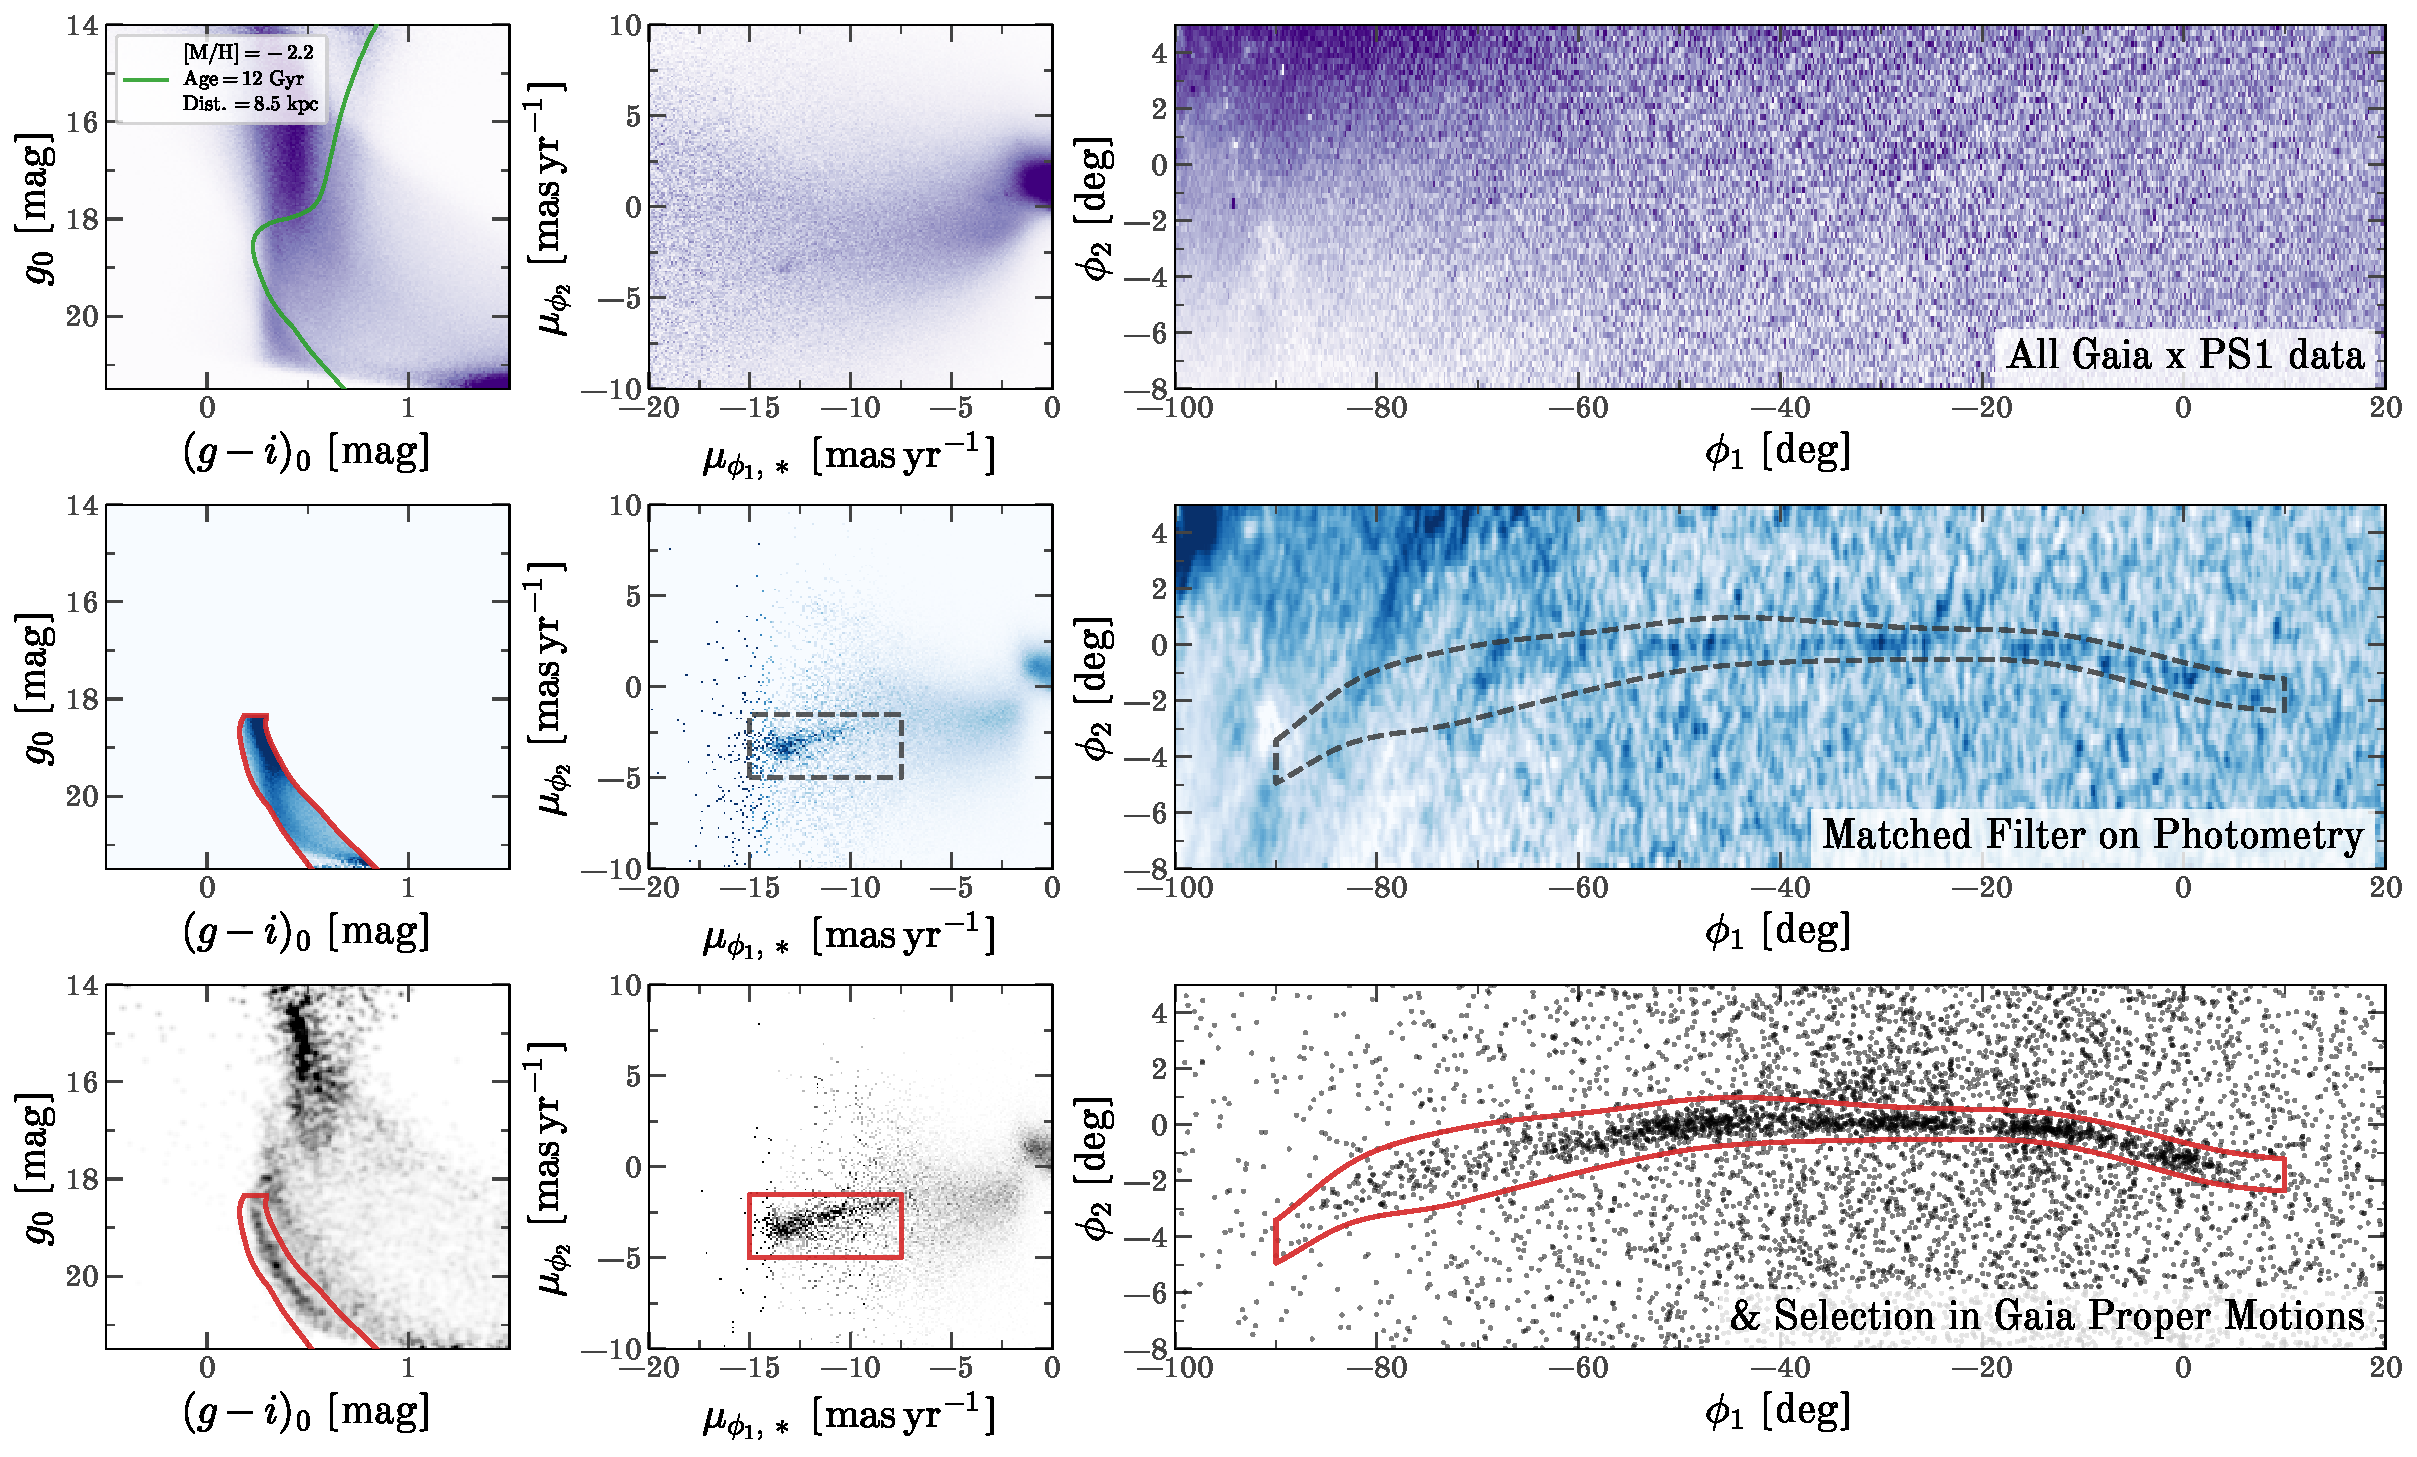
\includegraphics[width=1\textwidth]{gd1-filter-demo.pdf}
    \end{center}
    \caption{%
    TODO: Descriptive suptitle.
    A demonstration of how matched filtering with photometry and \gaia\ astrometry can
    be used to reveal a stellar stream, here the GD-1 stream.
    In all rows, the left panel shows an extinction-corrected color--magnitude diagram
    using $g, r, i$ photometry from the Pan-STARRS (PS1) survey \citep{chambers:2016},
    visualized as a row-normalized 2D histogram.
    The center panel shows the proper motions from \gaia\ \dr{3} \citep{gaiadr3}
    transformed into a coordinate system aligned with the stream, $(\mu_{\phi_1, *},
    \mu_{\phi_2})$, where $\phi_1$ is the stream longitude and $\phi_2$ is the stream
    latitude, and the color scale is a column-normalized 2D histogram.
    The right panel shows the sky positions of stars as a column-normalized 2D
    histogram.
    \textbf{Top row:} No selections have been applied: These panels show all stars in a
    cross-match between \gaia\ \dr{3} and PS1 for the region of the sky around the GD-1
    stream.
    \textbf{Middle row:} A binary matched filter has been applied to the photometry, as
    shown by the red polygon in the left panel of this row.
    Note that already the stream is visible as an over-density of stars in
    proper-motions (center panel) and in the known stream track (dashed line in the
    right panel).
    \textbf{Bottom row:} In a given panel, selections are applied based on the red
    outlines in the other two panels.
    For example, in the left panel, stars are shown as selected within the proper motion
    selection box (red outline in the center panel) and the sky track polygon (red
    outline in the right panel).
    \label{fig:gd1-demo}
    }
\end{figure*}

% TODO: Yanny? Others for list of SDSS stream papers?
Even now, many (TODO: how many?) of the known streams were found using a matched filter
based on photometry, plus visual inspection.
For example, the GD-1 stream --- the first long, thin stream discovered without a clear
progenitor --- was initially found by \citet{Grillmair:2006-gd1} using a matched filter
on SDSS photometry with visual inspection of the resulting stellar density maps.
Matched filters were also critical for many early discoveries of streams with the SDSS
data \citep[e.g.,][]{Newberg:2002, Yanny:2003, Belokurov:2006, Grillmair:2006-orphan}.
This method has since been applied to many large photometric surveys, such as 2MASS,
Pan-STARRS (PS1; \citealt{chambers:2016}), the Dark Energy Survey (DES;
\citealt{des:2005, des:2016}), the DECam Legacy Survey  (DECaLS; \citealt{dey:2019}),
the Pan-Andromeda Archaeological Survey (PAndAS; \citealt{mcconnachie:2009}),
and many smaller surveys.
In all cases, this has led to new stream and halo substructure discoveries.
For example, from 2MASS \citep{rocha-pinto:2003, rocha-pinto:2004}, PS1
\citep{bernard:2014, bernard:2016, navarrete:2017}, DES \citep{shipp:2018}, SLAMS
\citep{jethwa:2018}, PAndAS \citep{martin:2014}, and DECaLS \citep{shipp:2020}.
\todo{a table?} Table~\ref{todo} has a list of streams discovered ...

Many of the systematic searches for streams described above were done without
considering specific progenitor systems (i.e. globular clusters or dwarf galaxies).
The discovered streams were then subsequently either found to be without a clear
progenitor system, or were associated with known systems based on their location in the
sky and/or their kinematics.
However, some searches were specifically designed to find streams associated with known
globular clusters or dwarf galaxies \citep[e.g.,][]{grillmair:1995, kuhn:1996,
leon:2000} using photometry around these systems.
With the later exceptions of the striking tidal tails around the Pal 5 globular cluster
\citep{odenkirchen:2001} and the faint stream associated with NGC 5466
\citep{Grillmair:2006-ngc5466}, most of these searches were unsuccessful or only found
evidence for very low-density tidal tails based on the presence of small numbers of
extra-tidal stars around the progenitor systems \citep{grillmair:1995, leon:2000}.

The first stream discoveries and early theoretical work motivated the development of
new methods to identify lower surface brightness and more distant streams using a myriad
of techniques.
In most cases, however, searches for streams have focused on finding linear or curving
but ``thin'' stream features in projected sky coordinates.
For example, even before the first halo streams were found, it was recognized that tidal
debris from distant merger events should remain spatially coherent for many dynamical
times (gigayears, in the Milky Way halo; \citealt{johnston:1998, helmi:1999}).
From early numerical simulations, it was also noted that --- in a spherical or
nearly-spherical dark matter distribution --- the streams would phase mix almost along
great circles on the sky \citep{johnston:1996, Ibata:XXXX, others}.
This motivated the development of methods to search for over-densities of stars along
great circles in sky positions or photometrically-filtered sky positions of stars (the
``great circle cell count'', GC3, method; \citealt{johnston:1996}).
The GC3 method was used to identify and trace the extent of the Sagittarius stream using
2MASS data for M giant stars \citep{majewski:2003} and was later adapted to handle other
kinematic dimensions (the modified GC3 or ``mGC3'' method, which also uses proper motion
and radial velocity data; \citealt{Mateu:2011}).
The mGC3 method has since been used to identify many candidate stellar streams using RR
Lyrae-type stars \citep{Mateu:2018}.

Even in the pre-\gaia\ era, it was recognized that the kinematics of stars could be used
to search for streams and kinematic substructures in terms of dynamical invariants,
which would enable finding substructures that are not spatially coherent or so nearby
that they appear broad in sky projection.
For example, to identify potential streams or other dynamical structures in phase-space,
\citet{helmi:1999} used a small sample ($<100$) of metal-poor giant stars in the solar
neighborhood to search for kinematic over-densities of stars.
This early search for substructures in the solar neighborhood used astrometry from the
\hipparcos\ Mission \citep{perryman:1997} combined with literature measurements of
radial velocities of these stars to obtain full (6D) phase-space measurements of the
stars.
With 6D phase-space measurements, the stellar kinematics can be transformed into
integrals of motion (e.g., angular momentum) and Galactocentric velocity components,
where streams and other accreted tidal debris features are predicted to remain coherent
for longer than in position-space alone \citep{helmi:1999, sanderson:2015}.
Until recently, this was only possible with relatively small samples of stars with
precisely-measured astrometry, because the ability to identify clumps and over-densities
in dynamical or orbital quantities depends strongly on the precision of observed
kinematic coordinates and the number of stars.

\begin{figure*}[t!]
    \begin{center}
    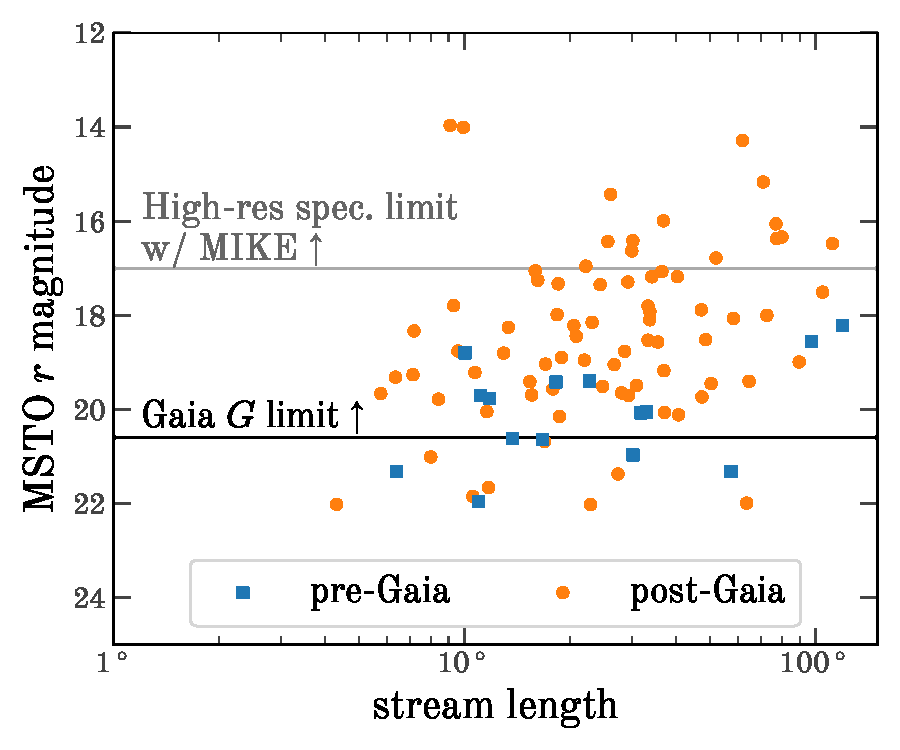
\includegraphics[width=1\textwidth]{msto-rc-mag.pdf}
    \end{center}
    \caption{%
    % TODO: add DES streams to left panel?
    Tracks of the apparent $r$-band magnitude of the main sequence turn-off (MSTO) for
    streams discovered before \gaia\ \dr{2} (left panel) and since (right panel).
    The tracks were determined by fitting orbits to stream stars associated with each of
    the streams in \citet{ibata:2024} (this procedure is described in detail in
    \ref{apx:stream-fit}).
    The MSTO magnitude is computed assuming all streams have a single stellar population
    with an age of $12~\unit{\giga\year}$ and a metallicity of $\feh = -2.2$, but this
    is only meant to qualitatively show the relative brightness of the MSTO for the
    known streams.
    High-resolution spectroscopic follow-up of MSTO stars in these streams is difficult
    or currently infeasible for many of these streams.
    RGB stars in the streams are typically bright enough for this type of follow-up, but
    are far less numerous than MSTO stars (globular cluster streams may only have a few
    to tens of RGB stars).
    \label{fig:msto-rc-mag}
    }
\end{figure*}

Prior to the \gaia\ Mission, only a handful of the discovered streams were followed up
and characterized with subsequent observations or surveys (for example, to obtain radial
velocities or detailed element abundance measurements for the constituent stars).
This was largely due to the fact that many of the streams discovered in deep photometric
surveys were faint and distant, and therefore difficult to observe spectroscopically.
In all but a few cases, the main sequence turn-offs (MSTO) of the streams are
sufficiently faint so that only the Red Giant Branch (RGB) or Horizontal Branch (HB)
stars were practically observable.
But the RGB and HB stars in many thin streams are sparse and often distributed over
large areas of the sky, making it difficult to obtain a large sample of stream stars.
As a demonstration of this point, the left panel of Figure~\ref{fig:msto-rc-mag} shows
the PS1 $r$-band magnitude tracks of the MSTO as a function of stream longitude for 7
streams discovered before \gaia\ \dr{2} that have since been identified using \gaia\
astrometry. To obtain precise and high signal-to-noise element abundance measurements
using existing facilities, stars typically had to be brighter than $r \lesssim
18~\textrm{mag}$ --- the MSTO for most streams known pre-\gaia\ were fainter than this
limit.
The stream tracks in Figure~\ref{fig:msto-rc-mag} were determined by either fitting
orbits to stream stars associated with each stream using data from \citet{ibata:2024}
(this procedure is described in detail in \ref{apx:stream-fit}), or for streams that are
not in \citet{ibata:2024}, we use the distance modulus tracks reported in
\citet{li:2022} combined with sky tracks collected from discovery or characterization
papers \citep{shipp:2018, fu:2018, shipp:2019, ferguson:2022, tavangar:2022}.

The \gaia\ Mission --- especially data from the second data release in 2018 --- has
since transformed the discovery, characterization, and follow-up efficiency of stellar
streams around the Milky Way.


\subsection{After \gaia\ Data Release 2}

The \gaia\ Mission released Data Release 2 (DR2) in April 2018 \citep{gaiadr2}, which
included astrometry and mean photometry for nearly 1.7 billion stars based on the first
22 months of observations.
This data was transformative for the study of Milky Way stellar streams and stellar halo
stars.
While parallax measurements for stars in most stellar streams and throughout most of the
stellar halo were too noisy to be useful, the proper motions provided key kinematic
information for many of these stars for the first time.
For example, consider a MSTO star for an old stellar population with absolute magnitude
$M_G \sim 4~\unit{\mag}$, at a distance of $d = 10~\kpc$ with a transverse velocity
typical of the Milky Way halo of $v_{\textrm{tan}} = 100~\kms$.
This star would have a true parallax of $\varpi = 0.1~\unit{\mas}$, a total proper
motion $\mu \approx 2.1~\masyr$, and an apparent magnitude of $G = 19~\unit{\mag}$.
For a star of this apparent magnitude in \gaia\ \dr{2}, a typical parallax uncertainty
$\sigma_\varpi \sim 0.4~\unit{\mas}$ and a typical proper motion uncertainty $\sigma_\mu
\sim 0.4~\masyr$.
This means that the parallax measurement is entirely dominated by the uncertainty, but
the proper motion still has an appreciable signal-to-noise ratio of $\mu / \sigma_\mu
\sim 5$.
The ability to use proper motions to identify members of stellar streams immediately
enabled detailed looks at previously-known streams and new methods for finding streams
in the Milky Way.

Proper motion data provided by \gaia\ has proven to be invaluable for studying the
density structure of stellar streams.
While matched filtering on photometry alone can reveal the presence of a stream, the
stream stars are often still relatively low signal-to-noise features over the background
stellar density, meaning that the stream density and any variations in the density is
typically not well constrained.
Soon after \gaia\ \dr{2}, \citet{price-whelan:2018} demonstrated the power of combining
photometric and kinematic data to identify stream members and measure the density of the
GD-1 stream.
Figure~\ref{fig:gd1-demo} is a recreation of the selections performed in
\citet{price-whelan:2018} but now using data from \gaia\ \dr{3} \citep{gaiadr3}.
As mentioned above, the top row of panels in Figure~\ref{fig:gd1-demo} shows photometry
from PS1 (top left panel), proper motions from \gaia\ \dr{3} (top center panel), and sky
positions (top right panel) for stars in the sky region near the GD-1 stream.
The middle row of panels shows the same data, but now with a matched filter applied to
the photometry.
The bottom row of panels shows the same data, but now with a matched filter applied to
the photometry and a selection on the proper motions (shown as a red box in the bottom
center panel).
The bottom right panel now shows the sky positions of individual stars that pass these
selections, which reveals more of the stream (especially at $\phi_1 \lesssim -55^\circ$)
and enables quantifying the magnitude of density variations and gaps present along the
stream track.
This new view of GD-1 also revealed features of the stream that were not visible in
previous filtered characterizations of the stream \citep{Grillmair:2006-gd1,
koposov:2010, deboer:2018}, which we discuss more below in Section~\ref{sec:structure}.
Many other studies have also used \gaia\ proper motions to study the structure of GD-1
\citep[e.g.,][]{malhan:2018, li-yanny:2018, huang:2019, deboer:2020, ibata:2020}, the
Orphan--Chenab stream \citep{koposov:2019}, the Helmi streams \citep{koppelman:2019},
the Jhelum stream \citep{bonaca:2019}, the Ophiuchus stream \citep{caldwell:2020}, along
with work that has modeled the density structure of many streams simultaneously
\citep[e.g.,][]{patrick:2022}.

Over the years leading up to \gaia\ \dr{2}, searches for new streams pushed deeper using
well-calibrated photometry from surveys like PS1 and DES, resulting in a steady and
continuous increase in the number of known streams.
Figure~\ref{fig:num-streams} shows the cumulative number of Milky Way stellar streams
reported in the literature as a function of time, as collated in the \texttt{galstreams}
\citep{mateu:2023} library and combined with the recent atlas of stream data from
\citet{ibata:2024}.
However, the kinematic data from \gaia\ has enabled a new and important validation step
for previously discovered streams.
While many streams have been re-discovered and studied in detail using \gaia\ data, a
number of streams that were previously reported in the literature have not been
re-identified with \gaia\ data.
\todo{Do we call these out in the table? PS1-A, Hyllus, etc.}
This is not totally unexpected, as many of the streams discovered in the pre-\gaia\ era
pushed to fainter magnitudes and larger distances, where the \gaia\ data is noisier
and/or only RGB stars in the streams may pass the faint limit of \gaia.

\begin{figure*}[t!]
    \begin{center}
    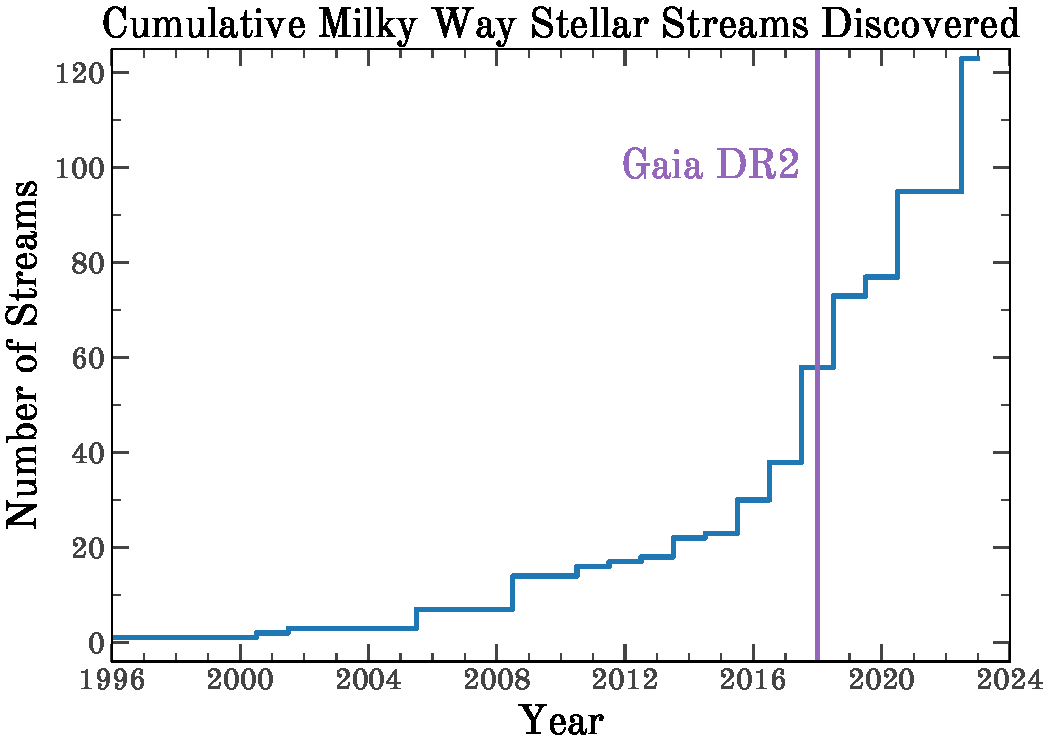
\includegraphics[width=0.6\textwidth]{cumulative-num-streams.pdf}
    \end{center}
    \caption{%
    TODO: Smoother rise. New data important, but also people refining methods and using smaller surveys along the way.
    \label{fig:num-streams}
    }
\end{figure*}

The exquisite astrometry provided by \gaia\ has also enabled a new class of methods for
searching for new streams around the Milky Way \citep[e.g.,][]{malhan:2018a,
borsato:2020, necib:2020, gatto:2020, shih:2022, shih:2023, pettee:2024}, which has led
to an enormous increase in the number of known low-density stellar streams.
These methods all leverage the kinematic data now available from \gaia\ to identify
over-densities of stars in different projections or transformations of the phase-space
data.
For example, \texttt{STREAMFINDER} \citep{malhan:2018a} searches for over-densities of
stars near orbits computed a model of the Milky Way's mass distribution.
This works by projecting orbits into the data space, where uncertainties and missing
data can be naturally handled by the search method.
Other methods either transform the phase-space data into a Galactocentric coordinate
system where clustering methods can search directly in the phase-space distribution
function \citep{necib:2020,gatto:2020}, or apply machine learning and anomaly detection
methods to the observed (heliocentric) data directly \citep{borsato:2020, shih:2022,
shih:2023, pettee:2024}.

The ability to use newly-accessible phase-space dimensions to search for streams has led
to the discovery of many low-density streams that would never have been found using
photometric selections alone.
For example, early work using \texttt{STREAMFINDER} identified a total of 13 new streams
in \gaia\ \dr{2} data \citep{malhan:2018, ibata:2018, ibata:2019}, which were typically
closer (and therefore appeared wider) and had lower surface densities than previous
photometrically-discovered streams.
This data has also enabled the discovery of streams that are not spatially coherent in
\emph{sky position} but do appear to contain comoving, metal-poor stellar populations
\citep[e.g.,][]{necib:2020b, balbinot:2023}.
Efforts have also searched for kinematic substructures that may be phase-mixed or less
spatially coherent using integrals of motion or other dynamical invariants
\citep[e.g.,][]{koppelman:2019b, yuan:2020, naidu:2020, ou:2023}.

The number of known stellar streams around the Milky Way has exploded in the \gaia\ era:
over 120 streams have now been reported in the literature (see
Figure~\ref{fig:num-streams}), with more discoveries coming every year, especially
enabled by new data releases from \gaia\ and new methodological developments.
\todo{Figure showing sky positions of all streams?}
With so many new streams, significant effort has been put into obtaining follow-up
spectroscopic observations of stream stars to measure their radial velocities and
detailed element abundances.
For example, surveys like the Southern Stellar Stream Spectroscopic Survey (S5;
\citep{li:2019,li:2022}) and more targeted efforts \citep[e.g.,][]{ibata:2021} are
steadily improving the validation and characterization of the current population of
known streams.
Future data releases from \gaia\ and new spectroscopic surveys and facilities such as
the Dark Energy Spectroscopic Instrument (DESI; \citealt{desi:2016}), H3
\citep{conroy:2019}, 4MOST \citep{4most:2012}, and WEAVE \citep{weave:2012} will
continue to enable new discoveries and detailed follow-up of the known streams.


\subsection{Key opportunities}
\begin{description}
    \item[Validation and spectroscopic characterization] Of all known streams...Many still need validation -- spectroscopy can be a challenge (see right panel of Fig blah)
    \item[Stream discovery in the disk plane and galactic center] Most streams at high latitude...see Figure~XXX, sky plot.
    \item[Automated discovery with quantified selection function] interpretation of population of observed streams in context of population of all streams hard because of selection effects. Contamination rate - requires observing (hard!) and publishing null results / non-discoveries.
    \item[Astrometry below the \gaia\ faint limit] Rubin, Roman
\end{description}

% - Deeper photometry - main sequence but more contamination from phot alone
%     - Combine with spectroscopy of full halo?


\section{Stream structure}
\label{sec:structure}
% APW
- Long known sagittarius bifurcation, no clear model to reproduce
- Now: Gaps and off-track features common at low surface brightness
- E.g., GD-1, Jhelum, AAU
- also motivated uncovering low-sb in other data sets (e.g., Pal 5, Jet, Phoenix)

- track--pm misalignments (shipp, erkal, ...)

\subsection{Key opportunities}
- density modeling robust to survey selection functions and dust



\section{Stream kinematics}
\label{sec:orbits}
% AB
- regime change: kinematics no longer painstaking follow-up, but part of discovery
- bulk for many streams \citep{streamfinders}
- individual follow-up as well \citep{others}
- galstreams summary: more streams w pm than not
-
% - census of papers w kinematics

\subsection{Orbits}
- a lot of what we want to do w streams is reconstructing their history
- depends on orbit!
- previously widely unknown (or rather, hard to get, so available for a few streams, but wildly unknown for most -- cite hermus hyllus stuff)
-- hermus \citep{grillmair:2014}
-- hermus, phoenix connection \citep{gc:2016}
-- bhb sdss velocities -> different orbit of hermus, not connected w phoenix \citep{martin:2018}

% - Still much unknown about most streams
- But Gaia gives us access to kinematics -> +MW model = orbits

-- orbital histories
-- satellite encounters

-- caveat: MW model
-- standard certainly idealized (LMC deformations)
-- fitting a more complex potential now possible (koposov student papers)


\subsection{Progenitors}
- progenitors important: can model much better (kupper)
- hard to find (balbinot)
- before: only 2 gc streams
- gjoll--ngc3201 chemistry \citep{hansen:2020}

- gaia: low sb bc selecting on orbits
- now a huge population, key opportunity

- orbits also connected separately identified streams
- case: oc
- case: aau \citep{li:2021}
- important for accurate accounting as we're moving to more complete census


\subsection{Population}
- orbital ensembles: used e.g., in Schwarzschild modeling of galaxy kinematics w individual stars, or updated inference on the MW mass w dwarf galaxies
- gaia for the first time allowed this for streams
- correlations present in MW satellites, e.g., VPOS
- streams orbital plane distribution, not aligned w the vpos \citep{riley:2020}

- more connections + benefit of orbits: phase-space clustering \citep{bonaca:2021}
- found origins (accreted vs in situ) + progenitor galaxies

- important for cocoon implications


\subsection{Chemistry}
- story of Monoceros, Anticenter Stream
-> thought accreted, but chemistry showed in-situ, kicked out of the disk

- chemistries even less available than radial velocities, need high-res, high snr spectra
- w Gaia: orbits good for better target selection, highly efficient targeting
-- S5 \citep{li:2022}
-- new streamfinder paper

- GC metallicity floor

- contribution of GCs

- origin of multiple populations, GD-1


\subsection{Key opportunity: Precision kinematics to determine the origin of stream perturbations}
- figure: progenitor, bar, gmc, dm subhalo (sky, vr - sampled 100m/s, pm - sampled GDR5)



\section{Outlook}
\label{sec:outlook}
- Due to more secure membership probabilities: follow-up now more efficient so the chemistries now becoming more readily available (ie stamp collecting more efficient)
- still sparse targets, but heavily multiplexed now
- desi already increasing samples
- weave, 4most imminent first light
- plug for cats, as a centralized repository??
% - More comprehensive spectroscopic follow-up, Stellar populations and element abundances -- save for the outlook

- Due to large number of streams: transitioning from stamp-collecting to population studies
% - comparison to surviving dwarf galaxies and clusters (internal properties and orbits) -- also mention in the outlook, as a part of building a complete picture

- All of this will need improved theoretical modeling of the new Gaia discoveries (+ outlook for the future)
% - potential modeling of a flexible potential -- also in the outlook

%% The Appendices part is started with the command \appendix;
%% appendix sections are then done as normal sections
\appendix

\section{Fitting Orbits to Streams}
\label{apx:stream-fit}

% for appendix
% Globular Cluster
% Code: PeTar
% Initial distribution function: King model, mass = 1e4 Msun, scaleradius = 4pc, w0=5. 50_000 particles.
% Particle masses: 0.2 Msun per particle
% PeTar handles collisional dynamics, so there is no softening. PeTar uses "slow-down algorithmic regularization (SDAR)" to calculate forces when particles have close passages.
%
% Dwarf Galaxy
% Code: Gyrfalcon
% Initial distribution function: King model, mass = 1e8 Msun, scaleradius = 1kpc, w0 = 4. 500_000 particles.
% Particle mass: 200 Msun per particle
% Softening epsilon = 0.01 kpc
% Energy errors are small, order 1e-5

We fit orbits to the 87 streams in the catalog of stream stars from \citet{ibata:TODO}
for demonstrative visualizations shown in this article.

For a given stream, we first determine a heliocentric, spherical coordinate system that
is approximately aligned with the stream track.
In this coordinate system, the stream longitude is $\phi_1$ and the stream latitude is
$\phi_2$.
We initialize this process by computing the eigenvectors of the covariance matrix of the
positions of the stream stars projected onto the unit sphere.
We project the unit vectors of the stream star positions onto the largest eigenvector
and use the endpoints along this axis to define an initial great circle coordinate
system.
We then adjust this great circle coordinate system by allowing small rotations around
the great circle $x$ and $y$ axes to minimize an objective function $F$ that computes
the sum of the squared stream latitudes, $\phi_2$: $F(\phi_2) = \sum_i \phi_{2,i}^2$ for
all stars in a stream, indexed by $i$.

To fit an orbit to each stream, we fix the model for the Milky Way's gravitational
potential to the \texttt{MilkyWayPotential2022} in \texttt{gala} \citep{gala} and
optimize over the orbital initial conditions.
We specify the orbital initial conditions in heliocentric coordinates in the rotated
stream coordinate system described above.
In this coordinate system, we define the orbital initial conditions at $\phi_1=0^\circ$,
so that the free parameters are the stream longitude, $\phi_2$, the distance, $D$, the
proper motion components, $(\mu_{\phi_1}, \mu_{\phi_2})$, and the line-of-sight
velocity, $v_r$.
For a given setting of the parameters $(\phi_2, D, \mu_{\phi_1}, \mu_{\phi_2}, v_r)$, we
integrate the orbit forward and backward in time, $\tau$, for an amount set by the
observed angular extent of the stream, $\Delta \phi_1$ divided by the transverse angular
velocity, $\sqrt{\mu_{\phi_1}^2 + \mu_{\phi_2}^2}$, and multiplied by two.
If the orbit wraps (over $360^\circ$), we truncate the orbit segment at $\phi_1 \pm
180^\circ$.

We then compute the log-likelihood of the orbit given the stream stars by assuming each
coordinate dimension is independent and normally distributed with a variance set by the
observational uncertainties.
In detail, we interpolate the orbit to the $\phi_1$ values of the stream stars using
cubic interpolation and compute the log-likelihood as:
\begin{equation}
\begin{split}
    \ln \mathcal{L} = \sum_i
    &\mathcal{N}(\tilde{\phi}_2(\phi_{1, i}) \given \phi_{2, i}, \sigma_{\phi_{2}}^2) \\
    \times \, &\mathcal{N}(\tilde{D}(\phi_{1, i})^{-1} \given \varpi_{i}, \sigma_{\varpi}^2) \\
    \times \, &\mathcal{N}(\tilde{\mu}_{\phi_1}(\phi_{1, i}) \given \mu_{\phi_1, i}, \sigma_{\mu_{\phi_1}}^2) \\
    \times \, &\mathcal{N}(\tilde{\mu}_{\phi_2}(\phi_{1, i}) \given \mu_{\phi_2, i}, \sigma_{\mu_{\phi_2}}^2) \\
    \times \, &\mathcal{N}(\tilde{v}_r(\phi_{1, i}) \given v_{r, i}, \sigma_{v_r}^2)
\end{split}
\end{equation}
where the tilde indicates the model predicted coordinates from the orbit and
interpolation step, evaluated at each stream star $\phi_{1, i}$, the distance component
is compared to the observed parallaxes $\varpi$, $\mathcal{N}(x \given \mu, \sigma^2)$
is the normal distribution with mean $\mu$ and variance $\sigma^2$, and the sum is over
all observed stars in the stream indexed by $i$.

We optimize the log-likelihood $\ln \mathcal{L}$ using the L-BFGS-B \citep{todo}
implementation in \texttt{scipy.optimize} \citep{scipy}, with bounds on the parameters
such that $\phi_2 \in (-5, 5)^\circ$, $D \in (1, 50)~\kpc$, $\mu_{\phi_1} \in (-100,
100)~\masyr$, $\mu_{\phi_2} \in (-100, 100)~\masyr$, and $v_r \in (-500, 500)~\kms$.
We start the optimization from six different initial distance values between $1~\kpc$
and $40~\kpc$ (spaced logarithmically) and take the optimized parameters from the run
with the highest log-likelihood value.
This process failed for TODO streams (TODO: stream names).

\bibliographystyle{model2-names-astronomy}
\bibliography{refs, apw-refs}

\end{document}

\endinput
%%
%% End of file `elsarticle-template-harv.tex'.
